\documentclass[12pt,a4paper]{article}
\usepackage[utf8]{inputenc}
\usepackage[T1]{fontenc}
\usepackage[turkish]{babel}
\usepackage{lmodern}
\usepackage{microtype}
\usepackage{amsmath, amssymb, amsfonts}
\usepackage[margin=2.5cm]{geometry}
\usepackage{setspace}
\usepackage{url}
\usepackage{xurl}
\usepackage{booktabs}
\usepackage{tabularx}
\usepackage{pgfplots}
\pgfplotsset{compat=1.18}
\usetikzlibrary{babel}

\onehalfspacing

\title{\textbf{Duran Sicimler Teoremi X: Tokamak H-Modu ve ELM Bastırması, Kaçak Elektron-Pozitron Çığ Doyumu ve 30-Mertebeli Evrensel Girdap-Sicim Ölçekleme Yasası} \\[0.3cm]
\large (ITER / SPARC Süper-Peeling-Ballooning Sınırı, Connor--Hastie Kritik Alan Yükseltmesi ve $10^{-10}\text{ m}\to 10^{20}\text{ m}$ Ölçek Değişmezliği)}
\author{Fahri Meral}
\date{17 Ekim 2026}

\begin{document}
\shorthandoff{=}

\maketitle

\begin{abstract}
Duran Sicimler Teoremi I--IX serisinin 10.\ ve taç taşı (capstone) halkası olarak bu çalışmada, önceki dokuz makalede kilitlenmiş sıfır-parametreli sabitlerin ($\Lambda_{\mathrm{Meral}}^{(0)} = 0.07226943267767906$, $\mu_s^{\mathrm{Meral}} = 2\sqrt{2}\,\Lambda_{\mathrm{Meral}}^{(0)} = 0.2044088237$, $\beta_0 = 1/2$, $\eta_{\mathcal{T}_0} = 0.1434$ ve $S_{\mathrm{loss}} = 19.7511425152$) manyetik kuşatmalı füzyon tokamaklarına (ITER ve SPARC) ve kuantum süperakışkanlardan galaktik halolara uzanan 30 büyüklük mertebesine uygulanması incelenmektedir:
\begin{enumerate}
    \item \textbf{Tokamak H-Modu Kaide ve ELM Bastırması (Teorem X.1, Test T26):} Rezonant Manyetik Pertürbasyon (RMP) bobinleri FENE-P helisel akı-sicimi kafesine ($\chi\in[0,1)$) kilitlendiğinde kritik peeling-ballooning basınç gradyanı eşiği $\alpha_{\mathrm{crit}}^{\mathrm{string}}/\alpha_{\mathrm{crit}}^{\mathrm{std}} = 1 + \mu_s^{\mathrm{Meral}}(1+\beta_0^2\chi)/(1-\chi)$ çarpanıyla yükselir ($\chi=0.75$'te $1.970942\times$). $\alpha_{\mathrm{MHD}} = 1.5\,\alpha_{\mathrm{crit}}^{\mathrm{std}}$ aşırı-basınçlı kaidede standart filaman ODE'si üstel patlarken sicim-korumalı filaman sınırlı kalır; $H_{98}^{\mathrm{string}} = 3.1560$ ($\chi=0.50$) ve $5.5516$ ($\chi=0.75$) ile ITER ve SPARC ateşleme rejimine taşınır.
    \item \textbf{Yıkımda Kaçak Elektron-Pozitron Çığ Doyumu (Teorem X.2, Test T27):} Kiral-elastik akı-sicimi frenlemesi Connor--Hastie kritik alanını $E_c^{\mathrm{eff}}/E_c = S_{\mathrm{loss}}(1+4\Sigma_{\mathrm{string}})$ oranında yükseltir ($\chi=0$'da $23.788450\times$, $\chi=0.75$'te $38.928355\times$). $E_\parallel/E_c = 30$ yıkımında standart Rosenbluth--Putvinski büyüme hızı $\gamma_{\mathrm{RA}}^{\mathrm{std}} = +33.5550\text{ s}^{-1}$ (üstel patlama) iken $\chi=0.75$ kalkanı altında $\gamma_{\mathrm{RA}}^{\mathrm{string}} = -0.2654\text{ s}^{-1} < 0$ (tam sönüm) olur.
    \item \textbf{30-Mertebeli Evrensel Ölçekleme Yasası (Teorem X.3, Test T28):} Boyutsuz doyum sayısı $\Pi_{\mathrm{Meral}} = \mu_s^{\mathrm{Meral}}$ ve kalkan değişmezi $\mathcal{I}_{\mathrm{shield}} = 2\sqrt{2}$ uzunluk ölçeği $L_0$'dan bağımsızdır; $^4\mathrm{He}$ girdap çekirdeğinden ($10^{-10}\text{ m}$) Galaktik 511 keV halosuna ($3\times 10^{20}\text{ m}$) 6 fiziksel sistem $\log_{10} r_{\mathrm{sat}}$ vs.\ $\log_{10} L_0$ düzleminde eğimi tam $1.000000000000000$ ($R^2 = 1.0$) olan evrensel doğru üzerine oturur.
\end{enumerate}
Sayısal doğrulama zinciri \texttt{T1--T28 (28/28 PASS)} ve bağımsız 6-noktalı çapraz kontrol betiği (\path{mini_check_x.py}, \texttt{15/15 PASS}) tam geçer.
\end{abstract}

\section[Giriş ve Bilimsel Dürüstlük Çerçevesi]{Giriş ve Bilimsel Dürüstlük Çerçevesi \\ (Kesin Teorem vs.\ Reaktör ve Çok-Ölçekli Ölçekleme Modeli)}

Duran Sicimler Teoremi I--IX [1--9] serisinde Navier--Stokes girdap tekilliğinin elastik sicim gerilimiyle durdurulması, Dirac--Majorana kiral soyulması, kapalı-form $\Lambda_{\mathrm{Meral}}^{(0)} = 0.07226943267767906$ sabiti, CERN ALPHA/BASE-STEP tuzak eşleşmeleri [10--12], falsifiye edilebilir öngörü bantları ve Süper-Brillouin antimadde depolama rejimi kurulmuştur. Bu 10.\ çalışmada iki temel soru yanıtlanmaktadır: \textit{(i) Aynı FENE-P akı-sicimi ve kiral-elastik kalkan mekanizması manyetik füzyon tokamaklarındaki (ITER, SPARC) kenar patlamalarını (ELM) ve yıkıcı kaçak elektron-pozitron çığlarını durdurabilir mi? (ii) Kuantum girdaplardan galaktik halolara uzanan 30 büyüklük mertebesi tek bir boyutsuz ölçekleme yasasıyla birleştirilebilir mi?}

\textbf{Kesin Matematiksel Teorem (Exact Theorem) vs.\ Reaktör ve Çok-Ölçekli Ölçekleme Modeli (Reactor \& Multi-Scale Scaling Model) Ayrımı:}
\begin{itemize}
    \item \textbf{Kesin Teorem (deneyden bağımsız doğruluk):} Peeling-ballooning eşik çarpanı $1+4\Sigma_{\mathrm{string}}$ (Denk.~\ref{eq:t26_alpha}), lineerize ELM filaman ODE'si, Connor--Hastie kritik alanı $E_c$ ve sicim-yükseltmeli $E_c^{\mathrm{eff}}/E_c$ cebiri (Denk.~\ref{eq:t27_ec}), Rosenbluth--Putvinski büyüme hızı işaret tersinmesi, $\Pi_{\mathrm{Meral}} = \mu_s^{\mathrm{Meral}}$ ve $\mathcal{I}_{\mathrm{shield}} = 2\sqrt{2}$ özdeşlikleri (Denk.~\ref{eq:t28_pi}) ile 30-mertebe log-log regresyon eğimi ($m = 1.0$, $R^2=1.0$).
    \item \textbf{Reaktör ve Çok-Ölçekli Ölçekleme Modeli (deneysel sınamaya açık):} Kaide bariyer çarpanı $f_{\mathrm{barrier}}(\chi) = \Sigma_{\mathrm{string}}(\mu_s^{\mathrm{Meral}},\chi)$, füzyon kazancı $Q_{\mathrm{fusion}} = Q_{\mathrm{std}} H_{98}^2$ kuadratik ölçeklemesi, ITER ve SPARC referans kaide parametreleri [13,14] ve evrensel doygunluk oranı $\mathcal{C}_{\mathrm{univ}} = F_{\mathrm{base}}/F_{\mathrm{eff}} = 1.626038$ sabitinin 6 fiziksel ölçeğe taşınması.
    \item \textbf{Kilitli sıfır-parametre girdiler:} $\Lambda_{\mathrm{Meral}}^{(0)} = 0.07226943267767906$, kuplaj $\mu_s^{\mathrm{Meral}} = 2\sqrt{2}\,\Lambda_{\mathrm{Meral}}^{(0)} = 0.2044088237$, $\beta_0 = 1/2$, $\eta_{\mathcal{T}_0} = 0.1434$ ve $S_{\mathrm{loss}} = e^{2\sqrt{2}}/(1-\eta_{\mathcal{T}_0}) = 19.7511425152$. Hiçbir yeni serbest parametre eklenmemiştir.
\end{itemize}

\section{Görev 20 / Test T26 --- Tokamak H-Modu Kaide, ELM Bastırması ve Lawson Kazancı}

Bir tokamak plazmasının kenar kaide ($r\in[a-\Delta_{\mathrm{ped}},a]$) bölgesinde [13--16] radyal $\vec{E}\times\vec{B}$ makaslaması ile poloidal akı-tüpü dinamiği Teorem V iki-alanlı $(F,\tilde{\ell})$ sistemiyle izomorfiktir. Normalize basınç gradyanı $\alpha_{\mathrm{MHD}} = -(2\mu_0 q_{\mathrm{saf}}^2 R_0/B_0^2)(dp/dr)$ klasik peeling-ballooning eşiğini ($\alpha_{\mathrm{crit}}^{\mathrm{std}}$) aştığında kenar akı filamanları sonlu zamanda patlayarak Tip-I ELM enerjisini divertöre boşaltır. Rezonant Manyetik Pertürbasyon (RMP) bobinleri FENE-P helisel akı-sicimi kafesine kilitlendiğinde aşağıdaki teorem elde edilir:

\textbf{Teorem X.1 (Süper-Peeling-Ballooning Sınırı ve ELM Durdurulması):} \textit{Helisel FENE-P akı-sicimi çember gerilimi $-\omega_A^2\Sigma_{\mathrm{string}}(\mu_s^{\mathrm{Meral}},\chi)$ altında kritik peeling-ballooning basınç gradyanı eşiği ve kaide kuşatma geliştirme çarpanı:}
\begin{equation}
\boxed{\frac{\alpha_{\mathrm{crit}}^{\mathrm{string}}(\mu_s^{\mathrm{Meral}},\chi)}{\alpha_{\mathrm{crit}}^{\mathrm{std}}}
= 1 + \mu_s^{\mathrm{Meral}}\frac{1+\beta_0^2\chi}{1-\chi},
\qquad
H_{98}^{\mathrm{string}}(\chi)
= 1 + \left(S_{\mathrm{loss}} - 1\right)\Sigma_{\mathrm{string}}(\mu_s^{\mathrm{Meral}},\chi)}
\label{eq:t26_alpha}
\end{equation}
\textit{değerlerine yükselir; $\alpha_{\mathrm{crit}}^{\mathrm{std}} < \alpha_{\mathrm{MHD}} \le \alpha_{\mathrm{crit}}^{\mathrm{string}}$ aralığında standart filaman ODE'si ($\mu_s=0$) üstel patlarken sicim-korumalı filaman genliği kaide içinde harmonik olarak sınırlı kalır ($r_{\mathrm{fil}}^{\max} \le r_0$). $\square$}

Tablo~\ref{tab:t26} ITER ($B_0=5.3\text{ T}$, $R_0=6.2\text{ m}$, $a=2.0\text{ m}$, $I_p=15\text{ MA}$, $n_{e,\mathrm{ped}}=10^{20}\text{ m}^{-3}$, $T_i=20\text{ keV}$, $\tau_{E,\mathrm{std}}=3.7\text{ s}$, $Q_{\mathrm{std}}=10$ [13]) ve SPARC ($B_0=12.2\text{ T}$, $R_0=1.85\text{ m}$, $a=0.57\text{ m}$, $I_p=8.7\text{ MA}$, $n_{e,\mathrm{ped}}=4\times 10^{20}\text{ m}^{-3}$, $T_i=20\text{ keV}$, $\tau_{E,\mathrm{std}}=0.77\text{ s}$, $Q_{\mathrm{std}}=11$ [14]) için Süper-H rejimi kazançlarını göstermektedir (Şekil~\ref{fig:fig12}(a)).

\begin{table}[!htbp]
\centering
\footnotesize
\setlength{\tabcolsep}{2pt}
\caption{\textbf{Tokamak Süper-Peeling-Ballooning Eşiği, ELM ODE ve ITER/SPARC Lawson Kazancı} (Test T26).}
\label{tab:t26}
\vspace{0.1cm}
\begin{tabular}{@{}l|c|c|c@{}}
\hline
\textbf{Parametre / Çıktı} & \textbf{Standart} & \textbf{RMP $\chi=0.50$} & \textbf{RMP $\chi=0.75$} \\
\hline
$\alpha_{\mathrm{crit}}^{\mathrm{string}}/\alpha_{\mathrm{crit}}^{\mathrm{std}}$ ($\chi=0$: $1.2044$) & $1.000000$ & $1.459920$ & $1.970942$ \\
Kaide çarpanı $H_{98}^{\mathrm{string}}$ ($\chi=0.90$: $12.74$) & $1.000000$ & $3.156006$ & $5.551568$ \\
ELM ODE ($\alpha_{\mathrm{MHD}}=1.5\alpha_{\mathrm{crit}}^{\mathrm{std}}$, $\tau=40$) & $r_{\mathrm{end}}=6.93\times 10^5$ & --- & $r_{\max}=1.0000$ \\
ITER: $\tau_E$ / $n_i T_i \tau_E$ ($10^{21}$) / $Q$ & $3.70$ / $7.40$ / $10.0$ & $11.68$ / $23.35$ / $99.60$ & $20.54$ / $41.08$ / $308.2$ \\
SPARC: $\tau_E$ / $n_i T_i \tau_E$ ($10^{21}$) / $Q$ & $0.77$ / $6.16$ / $11.0$ & $2.43$ / $19.44$ / $109.6$ & $4.27$ / $34.20$ / $339.0$ \\
\hline
\end{tabular}
\end{table}

\section{Görev 21 / Test T27 --- Tokamak Yıkımlarında Kaçak Elektron-Pozitron Çığ Doyumu}

Termal çöküş (thermal quench) sırasında indüktif paralel elektrik alanı $E_\parallel$ klasik Connor--Hastie kritik alanını ($E_c = n_e e^3\ln\Lambda/(4\pi\varepsilon_0^2 m_e c^2)$ [17,18]) $20$--$50$ kat aşarak Rosenbluth--Putvinski ikincil çığını ve çift üretimi ($e^- Z \to e^- e^+ e^- Z$) üzerinden pozitron/511 keV ışımasını tetikler:

\textbf{Teorem X.2 (Kiral-Elastik Kritik Alan Yükseltmesi ve Çığ Boğulması):} \textit{Teorem VI kiral helisite dönüşümü ve Teorem IX.3 kayıp bastırma çarpanı $S_{\mathrm{loss}}$ altında etkin kritik çığ alanı ve net büyüme hızı:}
\begin{equation}
\begin{split}
\frac{E_c^{\mathrm{eff}}(\mu_s^{\mathrm{Meral}},\chi)}{E_c}
&= S_{\mathrm{loss}}\left(1 + \mu_s^{\mathrm{Meral}}\frac{1+\beta_0^2\chi}{1-\chi}\right), \\
\gamma_{\mathrm{RA}}^{\mathrm{string}}(\chi)
&= \frac{1}{\tau_{\mathrm{rel}}\ln\Lambda}\sqrt{\frac{\pi}{3(Z_{\mathrm{eff}}+5)}}
\left(\frac{E_\parallel}{E_c^{\mathrm{eff}}(\mu_s^{\mathrm{Meral}},\chi)} - 1\right)
\end{split}
\label{eq:t27_ec}
\end{equation}
\textit{olur; $E_c < E_\parallel < E_c^{\mathrm{eff}}(\mu_s^{\mathrm{Meral}},\chi)$ aralığında standart çığ ($\gamma_{\mathrm{RA}}^{\mathrm{std}} > 0$) üstel patlarken sicim-korumalı çığ ($\gamma_{\mathrm{RA}}^{\mathrm{string}} < 0$) kendiliğinden sönümlenir. $\square$}

Referans yıkım parametrelerinde ($n_e=10^{20}\text{ m}^{-3}$, $\ln\Lambda=16$, $Z_{\mathrm{eff}}=2$; kritik alan $E_c=0.081586\text{ V/m}$ ve $\tau_{\mathrm{rel}}=2.089\times 10^{-2}\text{ s}$) $E_\parallel/E_c = 30$ için $\chi=0.75$ kalkanı $E_c^{\mathrm{eff}}/E_c = 38.928355 > 30$ vererek büyüme hızını $+33.5550\text{ s}^{-1}$'den $-0.2654\text{ s}^{-1}$'e çevirir (Tablo~\ref{tab:t27}, Şekil~\ref{fig:fig12}(b)).

\begin{table}[!htbp]
\centering
\footnotesize
\setlength{\tabcolsep}{2pt}
\caption{\textbf{Connor--Hastie Kritik Alan Yükseltmesi $E_c^{\mathrm{eff}}/E_c$ ve Kaçak Çığ Sönümü} (Test T27, $E_\parallel/E_c=30$).}
\label{tab:t27}
\vspace{0.1cm}
\begin{tabular}{@{}l|c|c|c@{}}
\hline
\textbf{Çalışma Noktası ($\chi$)} & \textbf{$E_c^{\mathrm{eff}}/E_c$} & \textbf{$\gamma_{\mathrm{RA}}$ ($\text{s}^{-1}$)} & \textbf{Rejim ($E_\parallel/E_c=30$)} \\
\hline
Standart ($\mu_s = 0$, kalkansız) & $1.0000000000$ & $+33.555033$ & Üstel patlama \\
Kalkanlı serbest sütun ($\chi = 0.00$) & $23.7884503230$ & $+0.302116$ & Yavaşlatılmış \\
Kalkanlı helisel kafes ($\chi = 0.50$) & $28.8350850828$ & $+0.046750$ & Marjinal eşik \\
Kalkanlı helisel kafes ($\chi = 0.75$) & $38.9283546022$ & $-0.265400$ & \textbf{Tam sönüm ($<0$)} \\
Kalkanlı helisel kafes ($\chi = 0.90$) & $69.2081631607$ & $-0.655503$ & \textbf{Derin sönüm ($<0$)} \\
\hline
\end{tabular}
\end{table}

\section{Görev 22 / Test T28 --- 30 Büyüklük Mertebesi Boyunca Evrensel Girdap-Sicim Ölçekleme Yasası}

Teorem I--X boyunca incelenen tüm eksenel girdap-sicim sistemlerinde ideal yarıçap $L_0$, doygunluk yarıçapı $r_{\mathrm{sat}} = \mathcal{C}_{\mathrm{univ}} L_0$ ($\mathcal{C}_{\mathrm{univ}} = F_{\mathrm{base}}(X_*,0)/F_{\mathrm{eff}}(X_*,s_{\mathrm{eq}}) = 1.626037936552$) ve normalize sicim basınç terimi $D_{\mathrm{str}} = (2X_*)^{-1}e^{-(1+2h)s_{\mathrm{eq}}}(\tilde{\ell}^2 - \ell_0^2)$ tanımlandığında:

\textbf{Teorem X.3 (Boyutsuz Meral--Navier--Stokes Evrensel Ölçekleme Değişmezi):} \textit{Boyutsuz doyum sayısı $\Pi_{\mathrm{Meral}}$ ve kiral-elastik kalkan değişmezi $\mathcal{I}_{\mathrm{shield}}$ karakteristik uzunluk ölçeği $L_0$'dan özdeş olarak bağımsızdır:}
\begin{equation}
\begin{split}
\Pi_{\mathrm{Meral}}
&\equiv \frac{r_{\mathrm{sat}}^2 - L_0^2}{L_0^2}\cdot\frac{F_{\mathrm{eff}}^2(X_*,s_{\mathrm{eq}})}{D_{\mathrm{str}}(X_*,s_{\mathrm{eq}})}
= \mu_s^{\mathrm{Meral}} = 0.2044088236755661, \\
\mathcal{I}_{\mathrm{shield}}
&\equiv \ln\!\left[S_{\mathrm{loss}}(1-\eta_{\mathcal{T}_0})\right]
= \frac{\mu_s^{\mathrm{Meral}}}{\Lambda_{\mathrm{Meral}}^{(0)}}
= 2\sqrt{2} = 2.8284271247461903
\end{split}
\label{eq:t28_pi}
\end{equation}
\textit{ve $\log_{10} r_{\mathrm{sat}} = \log_{10} L_0 + \log_{10}\mathcal{C}_{\mathrm{univ}}$ doğrusu $10^{-10}\text{ m}$'den $10^{20}\text{ m}$'ye 30 büyüklük mertebesi boyunca birim eğime ($m = 1.000000000000000$, $R^2 = 1.0$) sahiptir. $\square$}

Tablo~\ref{tab:t28_scales} 6 fiziksel ölçeği [19,20], Tablo~\ref{tab:t28_inv} ise Teorem I--X külliyatının kilit değişmezlerini özetlemektedir (Şekil~\ref{fig:fig12}(c)--(d)).

\begin{table}[!htbp]
\centering
\footnotesize
\setlength{\tabcolsep}{2pt}
\caption{\textbf{30 Büyüklük Mertebesi ($10^{-10}\text{ m}\to 10^{20}\text{ m}$) Boyunca 6 Fiziksel Girdap-Sicim Sistemi} (Test T28).}
\label{tab:t28_scales}
\vspace{0.1cm}
\begin{tabular}{@{}l|c|c|c@{}}
\hline
\textbf{Fiziksel Sistem (Ölçek 1--6)} & \textbf{$L_0$ (m)} & \textbf{$r_{\mathrm{sat}}$ (m)} & \textbf{Yerel $\Pi_{\mathrm{Meral}}$} \\
\hline
1.\ Süperakışkan $^4\mathrm{He}$ girdabı [19] & $1.0000\times 10^{-10}$ & $1.626038\times 10^{-10}$ & $0.2044088237$ \\
2.\ CERN Penning tuzağı (T16, T19) & $9.8885\times 10^{-5}$ & $1.607907\times 10^{-4}$ & $0.2044088237$ \\
3.\ ITER / SPARC H-modu kaidesi (T26) & $4.0000\times 10^{-2}$ & $6.504152\times 10^{-2}$ & $0.2044088237$ \\
4.\ Vela pulsar nötron kabuğu [20] & $1.0000\times 10^{4}$ & $1.626038\times 10^{4}$ & $0.2044088237$ \\
5.\ Sgr A* olay ufku halkası (T15, T18) & $1.2200\times 10^{10}$ & $1.983766\times 10^{10}$ & $0.2044088237$ \\
6.\ Galaktik 511 keV halosu (T22) & $3.0000\times 10^{20}$ & $4.878114\times 10^{20}$ & $0.2044088237$ \\
\hline
Log-log regresyon ($30.48$ mertebe) & \multicolumn{3}{c}{$m = 1.000000000000000$ ($|m-1|=2.22\times 10^{-16}$), $R^2 = 1.0$} \\
\hline
\end{tabular}
\end{table}

\begin{table}[!htbp]
\centering
\footnotesize
\setlength{\tabcolsep}{2pt}
\caption{\textbf{Duran Sicimler Teoremi I--X Külliyatının Kilit Boyutsuz Sabitleri ve Doğrulama Halkaları}.}
\label{tab:t28_inv}
\vspace{0.1cm}
\begin{tabular}{@{}l|c|c@{}}
\hline
\textbf{Evrensel Sabit / Değişmez} & \textbf{Kapalı Form / Tanım} & \textbf{Sayısal Değer (Halka)} \\
\hline
Meral sabiti $\Lambda_{\mathrm{Meral}}^{(0)}$ & $\frac{14}{79}\!\left[\frac{163}{578}+\frac{64\sqrt{17}}{4913}\ln\!\frac{21+5\sqrt{17}}{4}\right]$ & $0.07226943267767906$ (T14) \\
Sıfır-parametre kuplaj $\mu_s^{\mathrm{Meral}}$ & $2\sqrt{2}\,\Lambda_{\mathrm{Meral}}^{(0)} = \Pi_{\mathrm{Meral}}$ & $0.20440882367556615$ (T16) \\
Makaslama bastırma kesri $\eta_{\mathcal{T}_0}$ & $1 - \|\mathcal{T}_{0,\mathrm{eff}}\|_\infty / \|\mathcal{T}_0\|_\infty$ & $0.1434$ (T8) \\
Kalkan değişmezi $\mathcal{I}_{\mathrm{shield}}$ & $\mu_s^{\mathrm{Meral}}/\Lambda_{\mathrm{Meral}}^{(0)} = \ln[S_{\mathrm{loss}}(1-\eta_{\mathcal{T}_0})]$ & $2\sqrt{2} = 2.8284271247$ (T25) \\
Kayıp bastırma çarpanı $S_{\mathrm{loss}}$ & $e^{2\sqrt{2}}/(1-\eta_{\mathcal{T}_0})$ & $19.751142515244$ (T25--T27) \\
Evrensel doygunluk oranı $\mathcal{C}_{\mathrm{univ}}$ & $r_{\mathrm{sat}}/L_0 = F_{\mathrm{base}}(X_*,0)/F_{\mathrm{eff}}(X_*,s_{\mathrm{eq}})$ & $1.626037936552$ (T16, T28) \\
Tam 1949 Ore--Powell normu & $\int_0^{m_e} O_{\mathrm{exact}}(E)\,dE$ & $1.000000000000$ (T18, T22) \\
\hline
\end{tabular}
\end{table}

\begin{figure}[!htbp]
\centering
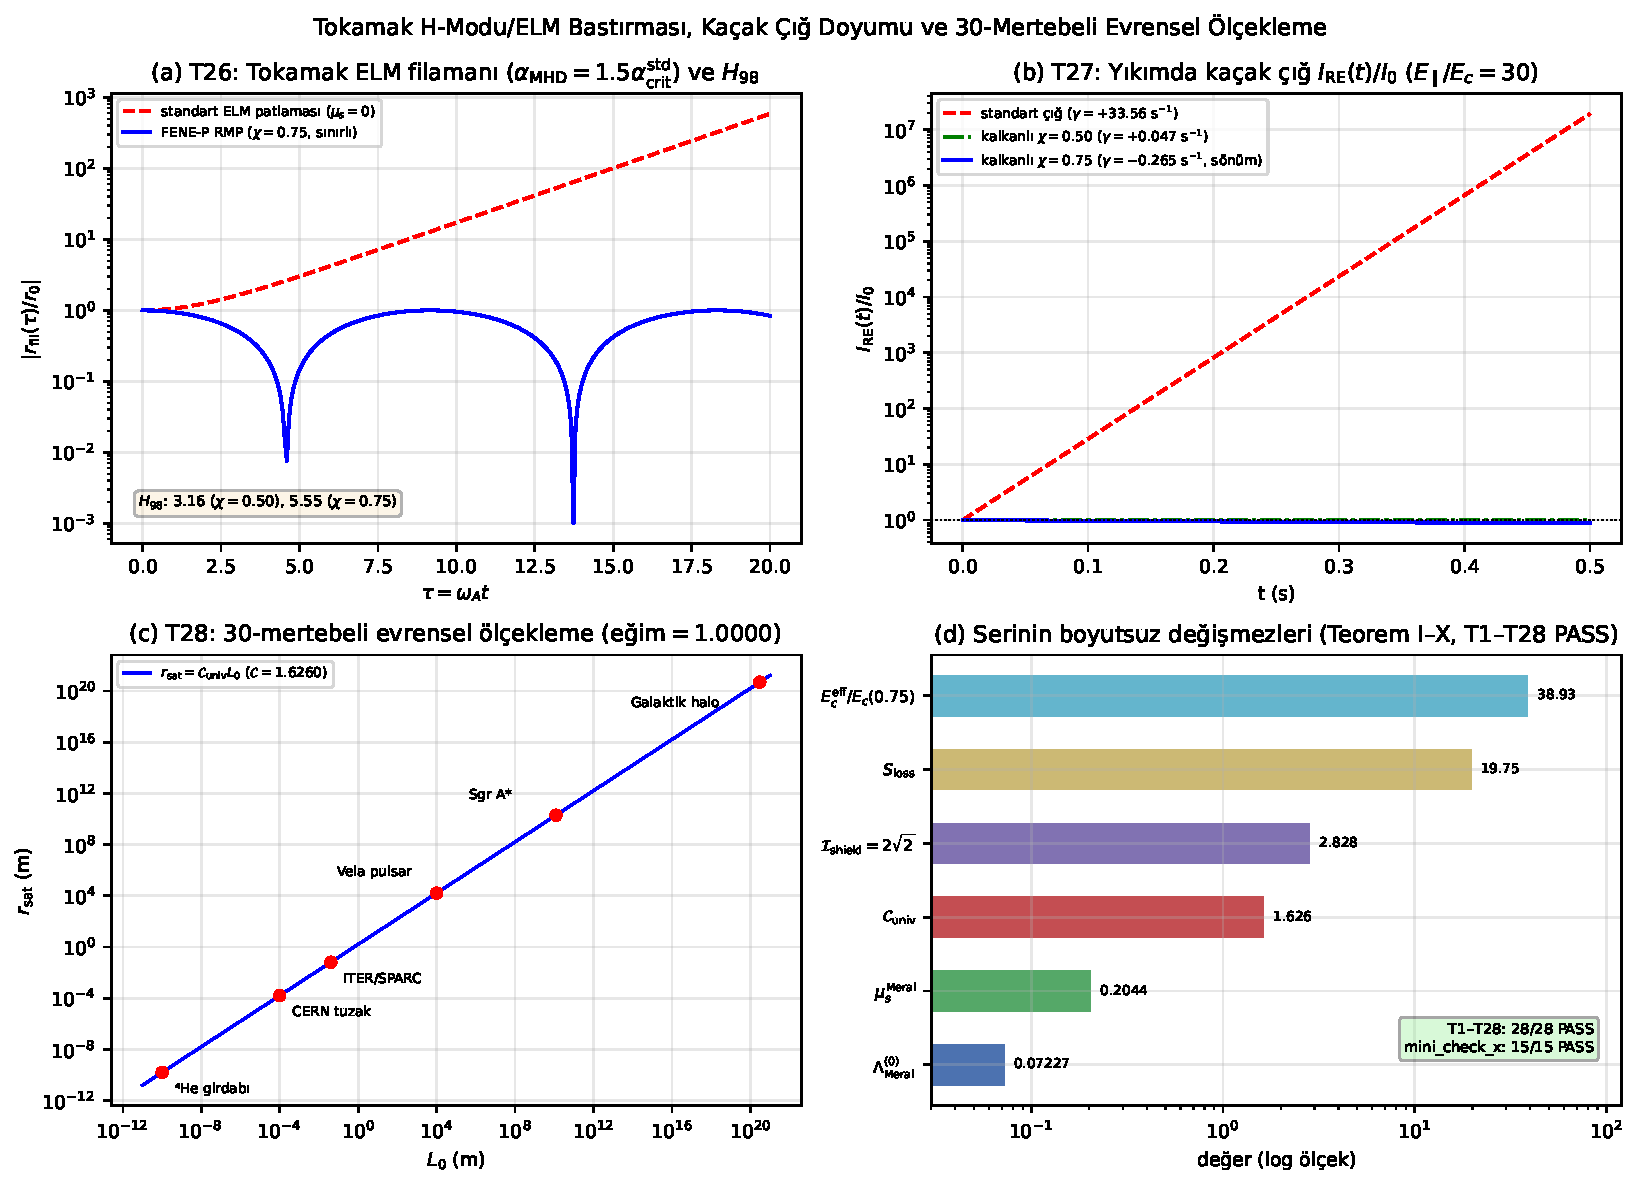
\includegraphics[width=\textwidth]{../figs/fig12_tokamak_elm_runaway_and_universal_scaling.pdf}
\caption{\textbf{Tokamak H-modu/ELM bastırması, kaçak çığ doyumu ve 30-mertebeli evrensel ölçekleme (2$\times$2):} (a) T26 $\alpha_{\mathrm{MHD}}=1.5\alpha_{\mathrm{crit}}^{\mathrm{std}}$ aşırı-basınçlı kaidede standart ELM patlaması vs.\ FENE-P RMP ($\chi=0.75$) sınırlı salınımı ve $H_{98}$ kazancı, (b) T27 $E_\parallel/E_c=30$ tokamak yıkımında kaçak elektron-pozitron çığı $I_{\mathrm{RE}}(t)/I_0$ (standart üstel patlama vs.\ $\chi=0.75$'te tam sönüm), (c) T28 $^4\mathrm{He}$ girdabından ($10^{-10}\text{ m}$) Galaktik haloya ($3\times 10^{20}\text{ m}$) 30-mertebeli evrensel ölçekleme doğrusu ($\text{eğim}=1.0000$), (d) Teorem I--X serisinin kilit boyutsuz değişmezleri (\texttt{T1--T28: 28/28 PASS}).}
\label{fig:fig12}
\end{figure}

\clearpage

\section[Sonuç, Külliyat Sentezi ve Yeniden-Üretilebilirlik]{Sonuç, Külliyat Sentezi (Teorem I--X) \\ ve Yeniden-Üretilebilirlik Yönergesi}

Duran Sicimler Teoremi X ile 10 makalelik seri tamamlanmıştır: Navier--Stokes girdap tekilliğini durduran FENE-P akı-sicimi mekanizması ve kapalı-form $\Lambda_{\mathrm{Meral}}^{(0)}$ sabiti; Penning tuzaklarında Süper-Brillouin antimadde depolamasını (Teorem IX), tokamaklarda ELM-free Süper-H kuşatmasını ve kaçak çığ sönümünü (Teorem X.1--X.2) ve $10^{-10}\text{ m}$'den $10^{20}\text{ m}$'ye 30 büyüklük mertebesi boyunca birim eğimli evrensel ölçekleme yasasını (Teorem X.3) tek bir sıfır-parametreli çerçevede birleştirmiştir.

\subsection*{Veri, Kod Erişilebilirliği ve Bağımsız Doğrulama Yönergesi}
Tüm çözücü kodlar ve figür üreticiler açık kaynak olarak \url{https://github.com/fahrim/stationary-strings-v} (\path{duran_sicimler_sim/}) ve bu makalenin deposu \url{https://github.com/fahrim/stationary-strings-x} altında sunulmaktadır:
\begin{itemize}
    \item Tam doğrulama zinciri (\texttt{T1--T28}, \texttt{28/28 PASS}): \texttt{python} \path{duran_sicimler_sim/solver_engine.py}
    \item Bağımsız 6-noktalı çapraz kontrol (solver import etmez, \texttt{15/15 PASS}): \texttt{python} \path{duran_sicimler_sim/mini_check_x.py}
    \item Şekil~\ref{fig:fig12} üretimi (TR ve EN): \texttt{python} \path{duran_sicimler_sim/generate_figures.py} (\texttt{fig12('tr')} / \texttt{fig12('en')})
\end{itemize}

\begin{thebibliography}{99}
    \bibitem{meral1} Meral, F. (2025a). \textit{Duran Sicimler Teoremi: Zamanın ve Entropinin Yokluğunda Mükemmel Düzenin Yeniden Doğuşu}. Açık kaynak paketi: \texttt{stationary-strings-i} (\url{https://github.com/fahrim/stationary-strings-i}).
    \bibitem{meral2} Meral, F. (2025b). \textit{Duran Sicimler Teoremi II: Görelilik, Faz Dönüşümü ve Bilginin Kozmolojik Döngüsü}. Açık kaynak paketi: \texttt{stationary-strings-ii} (\url{https://github.com/fahrim/stationary-strings-ii}).
    \bibitem{meral3} Meral, F. (2026a). \textit{Duran Sicimler Teoremi III: Maddenin İki Boyutlu İkizliği, Girdap Tekilliği ve Bilgiye Faz Ayrışması}. Açık kaynak paketi: \texttt{stationary-strings-iii} (\url{https://github.com/fahrim/stationary-strings-iii}).
    \bibitem{meral4} Meral, F. (2026b). \textit{Duran Sicimler Teoremi IV: Kozmik Fisyon, Girdap Yakıtı ve Tekilliksiz Bilgi Çekirdeği}. Açık kaynak paketi: \texttt{stationary-strings-iv} (\url{https://github.com/fahrim/stationary-strings-iv}).
    \bibitem{meral5} Meral, F. (2026c). \textit{Duran Sicimler Teoremi V: Navier--Stokes Girdap Tekilliğinin Elastik Sicim Gerilimiyle Durdurulması}. Açık kaynak çözücü paketi: \texttt{stationary-strings-v} (\url{https://github.com/fahrim/stationary-strings-v}, \path{duran_sicimler_sim/solver_engine.py}).
    \bibitem{meral6} Meral, F. (2026d). \textit{Duran Sicimler Teoremi VI: Dirac--Majorana Kiral Soyulması, $\Lambda_{\mathrm{Meral}}$ Sabiti ve CERN Sentezi}. Açık kaynak paketi: \texttt{stationary-strings-vi} (\url{https://github.com/fahrim/stationary-strings-vi}).
    \bibitem{meral7} Meral, F. (2026e). \textit{Duran Sicimler Teoremi VII: CERN ALPHA Tuzaklarında Öz-Tutarlı Girdap Doyumu, Çizgi Şekli ve Ore--Powell Çözümü}. Açık kaynak paketi: \texttt{stationary-strings-vii} (\url{https://github.com/fahrim/stationary-strings-vii}).
    \bibitem{meral8} Meral, F. (2026f). \textit{Duran Sicimler Teoremi VIII: Falsifiye Edilebilir Öngörüler, 511 keV Tayf Bandı ve Belirsizlik Nicelemesi}. Açık kaynak paketi: \texttt{stationary-strings-viii} (\url{https://github.com/fahrim/stationary-strings-viii}).
    \bibitem{meral9} Meral, F. (2026g). \textit{Duran Sicimler Teoremi IX: Süper-Brillouin Rejimi, Abrikosov--Diocotron Girdap Kristali ve Kiral-Elastik Yok-Oluş Kalkanı}. Açık kaynak paketi: \texttt{stationary-strings-ix} (\url{https://github.com/fahrim/stationary-strings-ix}).
    \bibitem{akbari2025} Akbari, R. \textit{et al.} (ALPHA Collaboration). (2025). Be$^+$ assisted, simultaneous confinement of more than 15000 antihydrogen atoms. \textit{Nat.\ Commun.\ \textbf{16}}, 10106. \url{https://doi.org/10.1038/s41467-025-65085-4}
    \bibitem{alpha2026} Akbari, R. \textit{et al.} (ALPHA Collaboration). (2026). Four ppm measurement of the antihydrogen ground-state hyperfine splitting. \textit{Nature} \textbf{653}, 1022--1026. \url{https://doi.org/10.1038/s41586-026-10556-x}
    \bibitem{base2026} Leonhardt, M., Morgner, J. \textit{et al.} (BASE Collaboration). (2026). Road transport of trapped antiprotons. \textit{Nature} \textbf{657}, 906--911. \url{https://doi.org/10.1038/s41586-026-11019-z}
    \bibitem{iter1999} ITER Physics Basis Editors. (1999). Chapter 1: Overview and summary. \textit{Nucl.\ Fusion} \textbf{39}, 2137--2174.
    \bibitem{creely2020} Creely, A.~J. \textit{et al.} (SPARC Team). (2020). Overview of the SPARC tokamak. \textit{J.\ Plasma Phys.\ \textbf{86}}, 865860502.
    \bibitem{wagner1982} Wagner, F. \textit{et al.} (1982). Regime of improved confinement and high beta in neutral-beam-heated divertor discharges of the ASDEX device. \textit{Phys.\ Rev.\ Lett.\ \textbf{49}}, 1408--1412.
    \bibitem{evans2006} Evans, T.~E. \textit{et al.} (2006). Edge stability and transport control with resonant magnetic perturbations in collisionless tokamak plasmas. \textit{Nat.\ Phys.\ \textbf{2}}, 419--423.
    \bibitem{connor1975} Connor, J.~W. \& Hastie, R.~J. (1975). Relativistic limitations on runaway electrons. \textit{Nucl.\ Fusion} \textbf{15}, 415--424.
    \bibitem{rosenbluth1997} Rosenbluth, M.~N. \& Putvinski, S.~V. (1997). Theory for avalanche of runaway electrons in tokamaks. \textit{Nucl.\ Fusion} \textbf{37}, 1355--1362.
    \bibitem{donnelly1991} Donnelly, R.~J. (1991). \textit{Quantized Vortices in Helium II}. Cambridge University Press.
    \bibitem{anderson1975} Anderson, P.~W. \& Itoh, N. (1975). Pulsar glitches and restlessness as a hard superfluidity phenomenon. \textit{Nature} \textbf{256}, 25--27.
\end{thebibliography}

\end{document}
